\documentclass{article}
\usepackage{amsmath,amssymb,tikz}
\begin{document}
Inline formula: $\frac{x^2+y^2}{2}$.
\[
  J=\sum_{k=0}^{N-1}\left(x_k^\mathsf{T}Qx_k+u_k^\mathsf{T}Ru_k\right)
\]
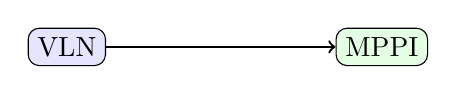
\begin{tikzpicture}
  \node[draw,rounded corners,fill=blue!10] (a) at (0,0) {VLN};
  \node[draw,rounded corners,fill=green!10] (b) at (4,0) {MPPI};
  \draw[->,thick] (a) -- (b);
\end{tikzpicture}
\end{document}
